\subsubsection{Recipe} \label{RecipesSketches}
In this section the recipe screen is going to be described. Both the functionality of the screen and the design principles used in the design process are going to be described. The sketch used to illustrate the use consist of two different screens, one screen only showing a full screen of the recipe, and one screen showing how to browse through the recipe. The browsing screen is divided into two sketches, showing the functionality of this screen.

The image sketches referred to can be seen in \cref{FinalRecipeBrowsingSketch2} and in \cref{FinalRecipeBrowsingSketch1}. The sketch in \cref{FinalRecipeBrowsingSketch1} is the first screen to see, when browsing recipes. The right screen in \cref{FinalRecipeBrowsingSketch2} shows the expanded version of the recipe browsing screen, and the left shows the full screen of the recipe.

\begin{figure}[H]
    \centering
    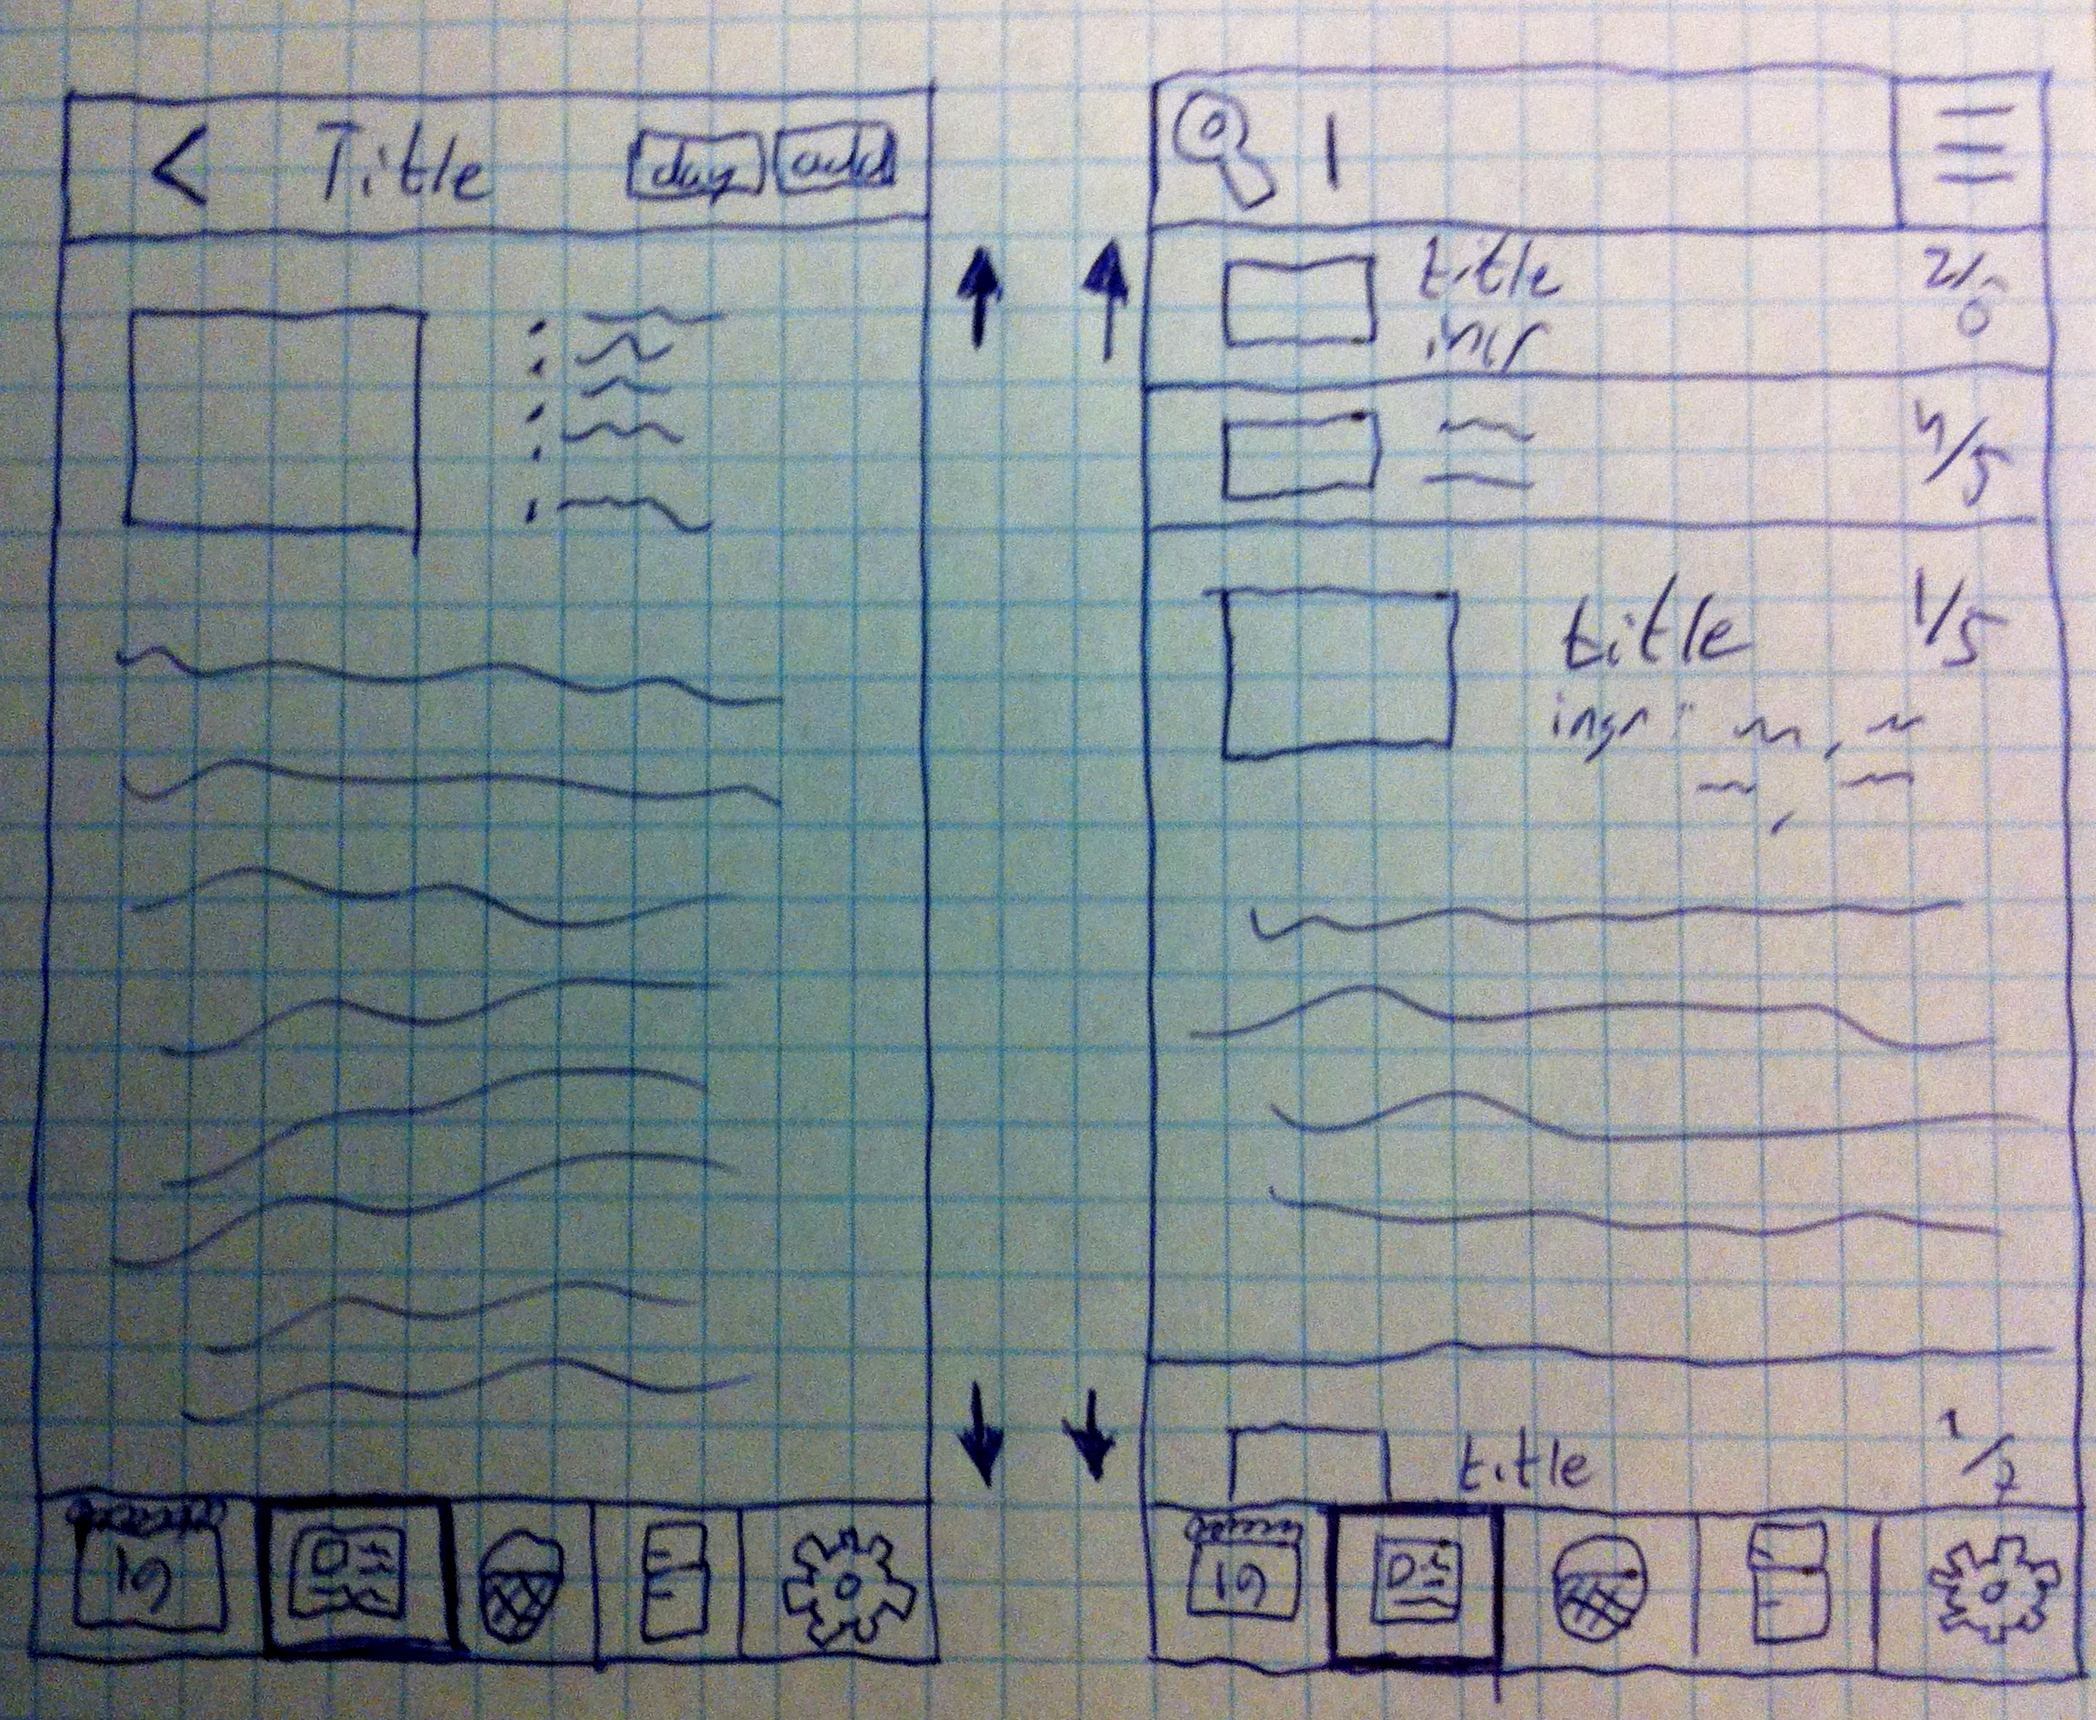
\includegraphics[width=0.5\textwidth]{Grafik/FoodPlanner/FinalRecipeBrowsingSketch2}
    \caption{One of the final sketches of the recipe browsing screen.}
    \label{FinalRecipeBrowsingSketch2}
\end{figure}

\textbf{Two screen idea:} Looking at the recipe browsing screen (right sketch on \cref{FinalRecipeBrowsingSketch2}) there are three elements to explain: 

\begin{itemize}
    \item Search bar
    \item Sort button
    \item List of recipes
\end{itemize}

The search bar is located on the top of the screen, as it is where the user is most likely to look for it at first, since this is where most search bars in mobile applications, but also websites, is located. When text is entered into the search bar, the recipes containing the text will be shown in the list of recipes. 

The sort button offers the user the functionality of sorting the list of recipes by different requirements. It might be by time to cook, by number of ingredients the user already has in the inventory, or by something else. The sort button is located at the right side of the search bar, as this was a convenient place to position it. It only consists of an icon showing that you will be able to sort the recipes by clicking the button.

The list of recipes show the recipes that the user can choose from. These are sorted by the sort button, or the search bar previously described. If there are more recipes available than the screen can display, the user will be able to swipe in an upwards motion for more recipes to appear at the bottom and the recipes at the top will disappear. In the right side of each recipe it is shown how many of the ingredients needed to make the recipe the user already have; an example is if the user has 4 out of the 10 ingredients needed the right side will show "4/10".

Looking at the specific recipe screen (left sketch on \cref{FinalRecipeBrowsingSketch2}) there are two elements to explain:

\begin{itemize}
\item Top navigation bar
\item Recipe viewing area
\end{itemize} 

The expanded recipe screen can be seen in \cref{FinalRecipeBrowsingSketch2} on the right. It is similar to the recipe browsing screen, but this screen shows more information about a specific recipe.

When the user has chosen a recipe, the user will be able to click it. By doing so, the recipe will expand, and more information about the recipe will be shown. This will only be the most relevant information, such as ingredients, cooking time, and a picture.

\begin{figure}[H]
    \centering
    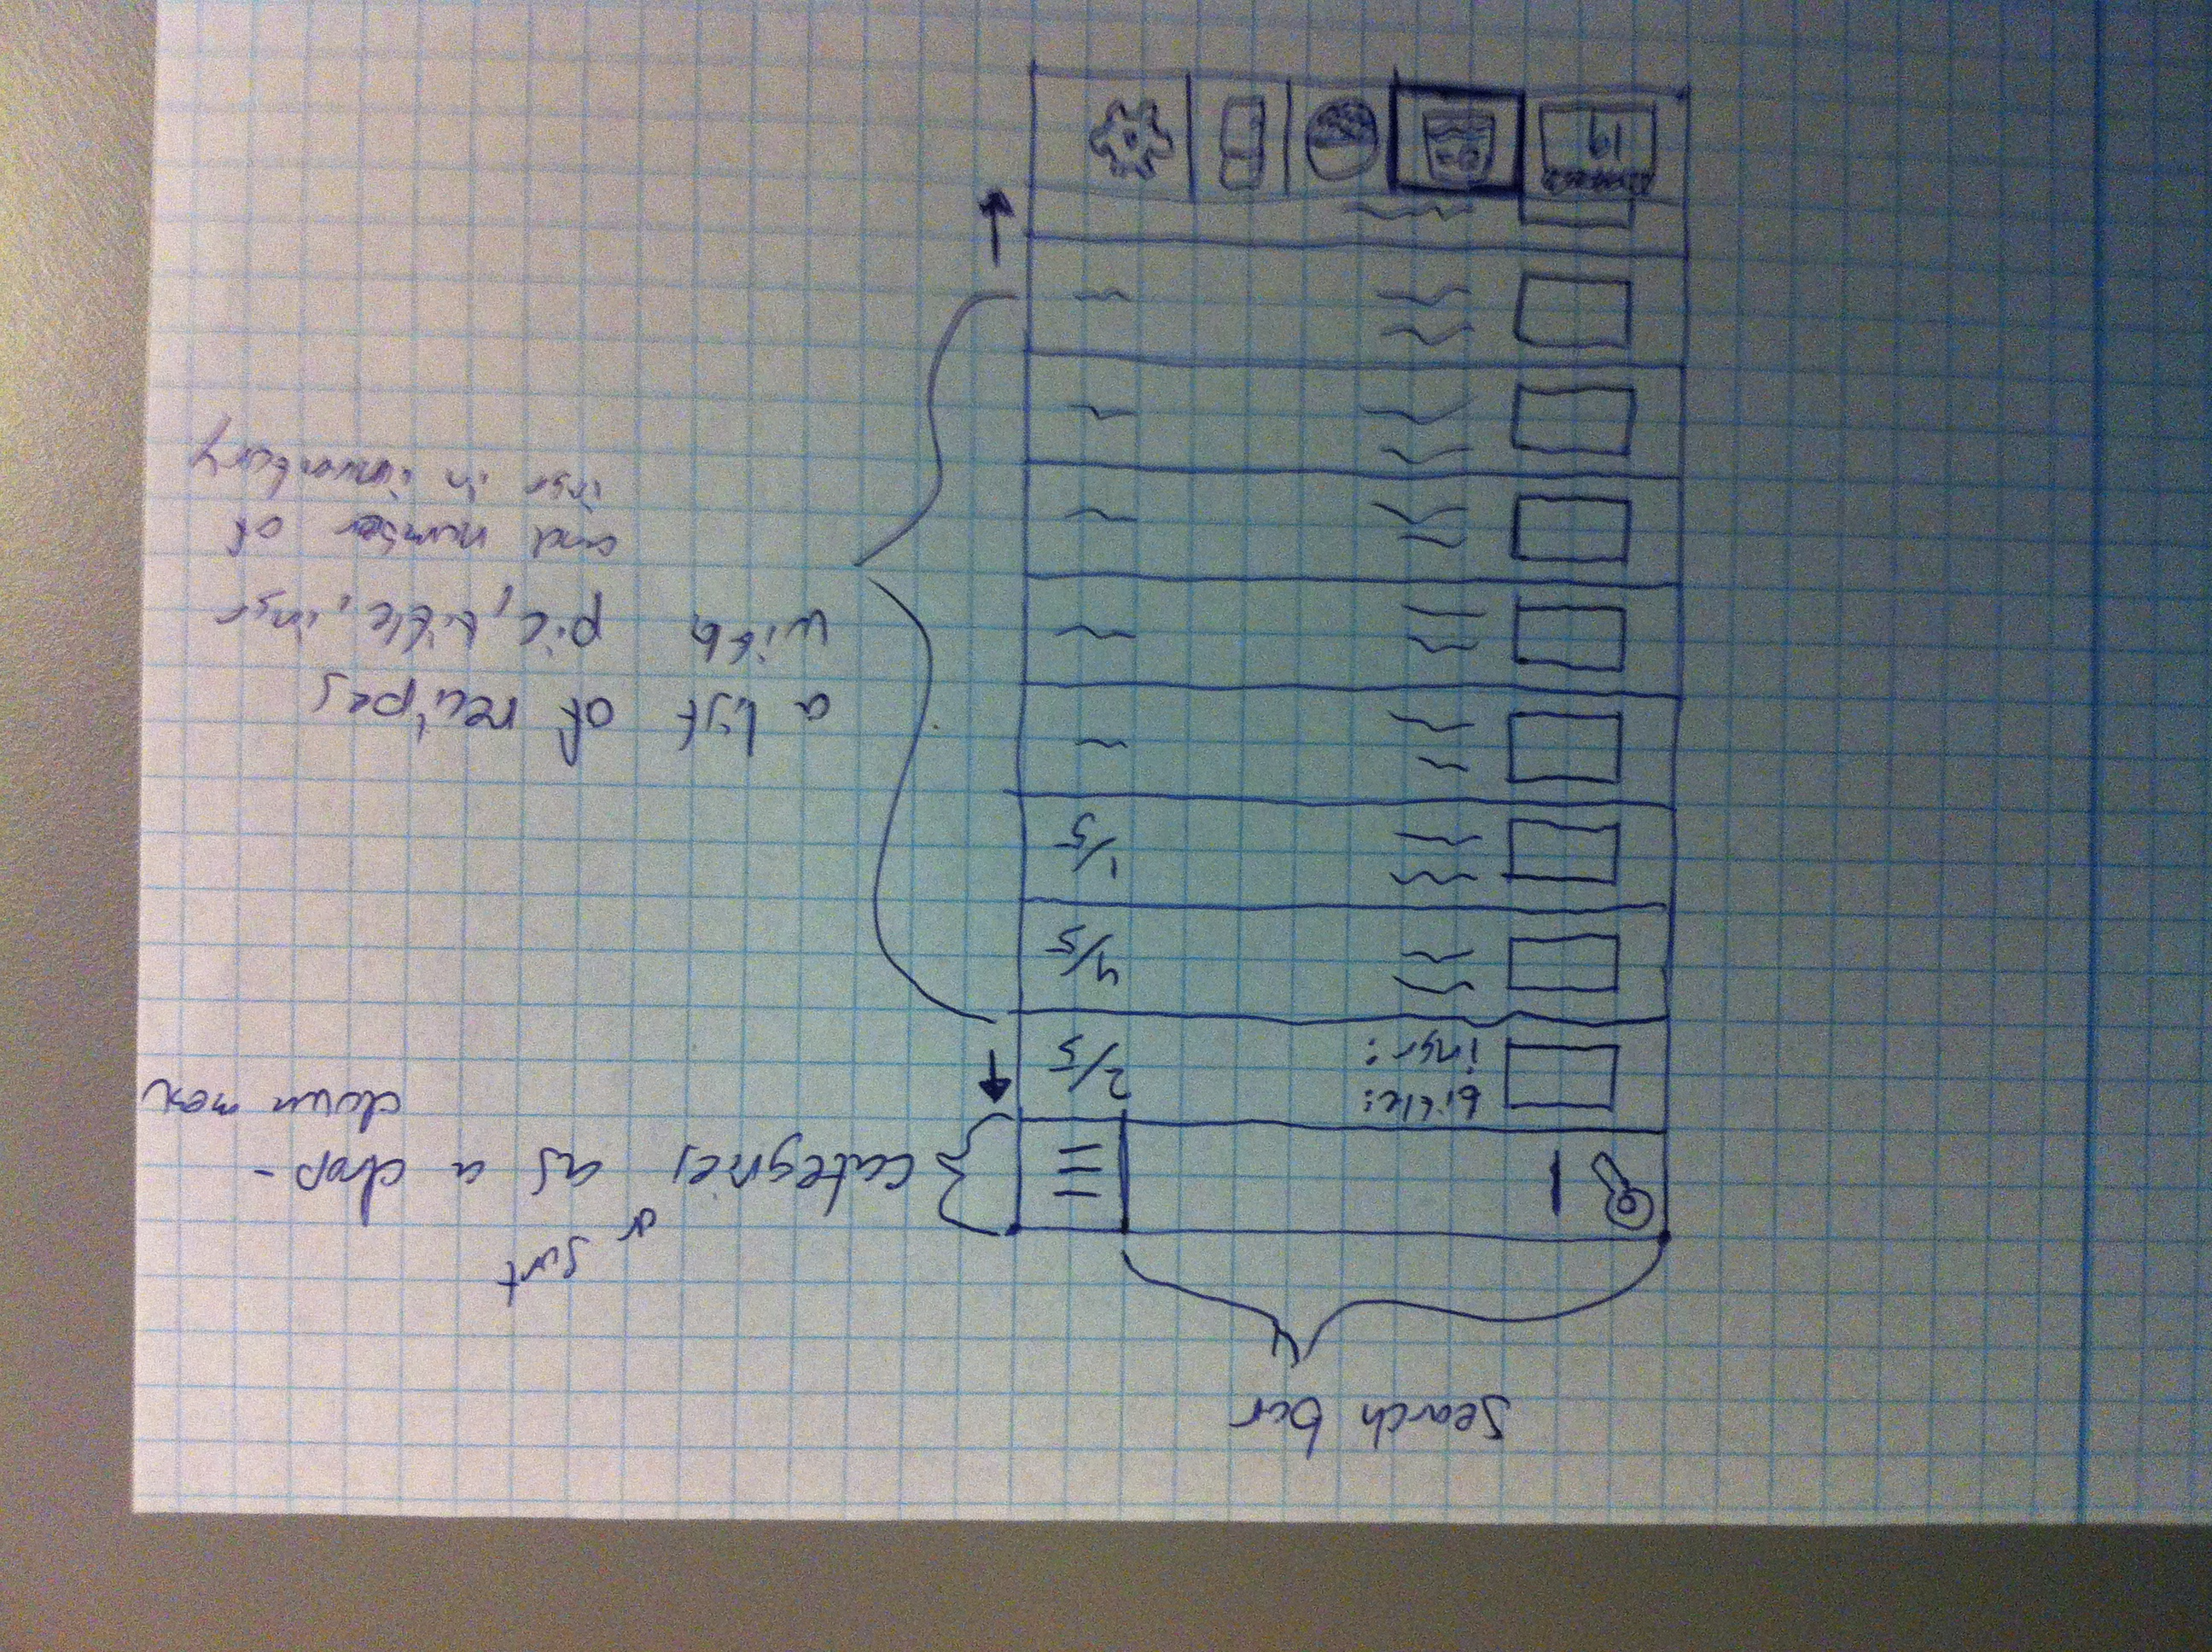
\includegraphics[width=0.5\textwidth]{Grafik/FoodPlanner/FinalRecipeBrowsingSketch1}
    \caption{One of the final sketches of the recipe browsing screen.}
    \label{FinalRecipeBrowsingSketch1}
\end{figure}

\textbf{Full screen recipe screen:} The full screen recipe screen is the left sketch on \cref{FinalRecipeBrowsingSketch2}. This screen gives the full overview of the recipe.

On the left side, a picture of the recipe will be shown if available, and the ingredients will be listed on the right side of the picture. Beneath the ingredient list, instructions on how to prepare the meal are shown. If the recipe is longer than the amount of text the screen can hold, the user will be able to scroll through the rest of the recipe by swiping.

In the top of the screen there is a navigation bar. This navigation bar gives the user the ability to do three things:

\begin{itemize}
    \item Go back
    \item Change the amount of people attending the meal
    \item Add the recipe to the meal plan
\end{itemize}

The arrow in the left of the navigation screen indicates a go back function, giving the user the ability to go back to the recipe browsing screen, if the user did not want to do anything further with the shown recipe.

The second element enables the user to change the amount of people attending the meal. This would change the amount of ingredients needed in the recipe, and would also update the shopping list, so the user would buy the right amount of the ingredients needed.

The last button gives the user functionality to add the recipe, being viewed, to the meal plan. This would update the shopping list, and add the meal to a specific day chosen by the user.